% Project Report for ME-F377 Project Course
\documentclass[11pt]{report}

\topmargin=0.0in
\oddsidemargin=0.0in
\evensidemargin=0in
\textwidth=6.5in
\marginparwidth=0.5in
\headheight=0pt
\headsep=0pt
\textheight=9.0in

\usepackage{amsmath}
\usepackage{amsfonts}
\usepackage{hyperref}
\usepackage{geometry,color,graphicx}
\usepackage{subcaption}
\usepackage{listings}
\usepackage{ff++listings}
\usepackage{pgf}
\usepackage{epstopdf}

\newtheorem{theorem}{Theorem}
\newtheorem{example}{Example}[chapter]
\newtheorem{result}{Result}[chapter]

\begin{document}
	\begin{titlepage}
		\begin{center}
			{\Large A Report}\\[1cm]
			{\Large On}\\[1cm]
			{\LARGE \textbf{Numerical Solutions to Partial Differential Equations using FEniCS}}\\[1cm]
			{\Large Prepared in partial fulfillment}\\[1cm]
			{\Large of}\\[1cm]
			{\Large \textbf{Design Project}}\\[0.5cm]
			{\Large \textbf{ME F377}}\\[1cm]

			{\Large By}\\[1cm]
			{\Large Sanath Keshav}\\[0.1cm]
			{\Large 2013A4PS359G}\\[0.3cm]

			\begin{figure}[h]
				\centering
				
\includegraphics[scale=0.7]{bits_logo.png}
			\end{figure}

			\textsc{BIRLA INSTITUTE OF TECHNOLOGY AND SCIENCE, PILANI}
		\end{center}
	\end{titlepage}

	\chapter*{Acknowledgements}
I would like to express my deepest appreciation to all those who helped me to complete this report. A special gratitude I give to my mentor Dr. P Dhanumjaya , for giving me this opportunity to work on this topic and also for his guidance and unwavering support during the whole semester. I would also like to particularly thank my classmate K Balaje for his constant support and motivation the whole time.
	\tableofcontents

	\chapter{Introduction}
	% $DOP/Report/chapters/introduction.tex
\hspace{5mm}In this report we introduce FEM for some elliptic model problems and study the basic properties of the method. We first consider a simple one-dimensional problem and then some two=dimensional generalisations. Consider the following \emph{model problems} - 
\begin{eqnarray}\nonumber
	&\text{1D: }&\qquad -u''(x) = f(x), \quad 0<x<1, \quad u(0) = u(1) = 0\\\nonumber
	&\text{2D: }&\qquad-\Delta u(x,y) = f(x,y), \quad (x,y) \in \Omega, \quad u(x,y)|_{\partial \Omega} = 0  
\end{eqnarray}
where $\Delta$ denotes the \emph{Laplacian} operator, $\Omega$ is the domain in the $(x,y)$ plane with the boundary $\partial \Omega$.

\section{Preliminaries}

We now introduce some notation that will be used below. We define
\begin{equation}
D^\alpha v = \frac{\partial ^{|\alpha|} v}{\partial x_1^{\alpha_1} \partial x_2^{\alpha_2} \dots \partial x_n^{\alpha_n}}
\end{equation}
where here $\alpha = (\alpha_1,\alpha_2), \alpha_i $ is a non-negative natural number and $|\alpha| = \alpha_1 + \alpha_2$. As an example, a partial derivative of order 2 can there be written as  $D^\alpha v $ with $\alpha=(2,0), \alpha = (1,1)$ or $\alpha =(0,2), $ which are the$\alpha$ with $|\alpha| = 2$.

We now define for $k = 1,2, .... ,$
\begin{equation}
H^k(\Omega) = \Big\{ u(x) \ \Big| \ D^\alpha u \in L^2(\Omega), \ |\alpha|\le m   \Big\}
\end{equation} 

\subsection{The Hilbert spaces}
When giving the variational forms of the boundary value problems for partial differential equations, it is from the emathematical point of view natural and very useful to work with function spaces V that are slightly larger than the spaces of continuous functions with piecewise continuous derivatives. It is also useful to endow the spaces V with various scalar products with the scalar product related to the boundary value problem. More precisely, V will be a Hilbert space.

We now introduce some Hilbet spaces that are natural to use for variational formulations of the boundary value problems we will consider. Let us start with the one-dimensional case. If $I = (a,b)$ is an interval, we define the space of "square integrable functions" on I :
\begin{equation}
L^2(I) := \bigg\{ v:  \int_{I} v^2(x) \ dx < \infty\bigg\}
\end{equation}
with the norm:
\begin{equation}
\lVert v \rVert_{L^2} := \bigg( \int_{I} v^2 \ dx \bigg)^{1/2}.
\end{equation}

The space $H^1(I)$consists of the functions v defined on I which together with their first derivatives are square integrable, ie, belong to $L_2 (I)$
\begin{equation}
H^1(I) = \Big\{ v \ \Big| \ \int_{I} v^2 \ dx < \infty, \ \int_{I} (v')^2 \ dx < \infty \Big\}
\end{equation}
\begin{equation}
H^1(\Omega) = \Big\{ v(x,y) \ \Big| \ v \in L^2(\Omega), \ \frac{\partial v}{\partial x} \in L^2(\Omega), \ \frac{\partial v}{\partial y} \in L^2(\Omega) \Big\}
\end{equation}
We equip this space with the scalar product 
\begin{equation}
(v,w)_{H^(I)} = \int_{I} (vw + v'w')dx
\end{equation}
\begin{equation}
\lVert v \rVert_{H^1} := \bigg( \int_{I} (v^2 + v'^2) \ dx \bigg)^{1/2}.
\end{equation}
In case of boundary value problems of the form  $ -u'' = f$ on $ I = (a,b)$ with boundary conditions $u(a) = u(b) = 0$, we shall use the space
\begin{equation}
H^1 _0(I) = \Big\{ v \in H^1(I): v(a)=v(b)=0\}
\end{equation}
with the same scalar product and norm as for $H^1(I)$.

	
	\chapter{1D Elliptic Problems}
	% Report/chapters/1d.tex
\hspace{5mm}In this chapter, we will consider the following boundary value problem for the poisson equation and demonstrate how the Finite Element Method can be implmented in MATLAB to compute the solutions to different Ordinary Differential Equations subjected to \textbf{Dirichlet, Neumann and Robin} Boundary Conditions.
\section{Weak formulation}
\hspace{5.4mm}Consider the \emph{2-Point Boundary Value Problem} in 1D,
\begin{eqnarray}
-u''(x) &=& f(x) \quad \text{in} \quad \Omega \equiv (0,1)\label{model}\\
u(0) &=& u(1) \ \ = \ \ 0
\end{eqnarray}
Now, let us look at the general procedure that is usually followed to find out the \textbf{Finite Element Solution} of the problem.

\begin{enumerate}
	\item \textbf{Derive the Variational/Weak Formulation}:
	We shall now give an abstract formulation of the finite element method for elliptic problems. This makes it possible to give a unified treatment of many problemsin mathematics and physics. Considering the Galerkin Approach, we construct the weak formulation of our \textbf{2-Point BVP} by multiplying both sides of \ref{model} with a \textbf{test function} $v$ satisfying $v(0) = v(1) = 0$ and integrating it over the domain $\Omega \equiv (0,1)$ .
	\begin{equation}
	-\int_{0}^{1} u'' v\ dx = \int_{0} ^{1} fv \ dx
	\end{equation}
	\begin{equation}
	- \ u'v \ \Big|_0^1 + \int_{0}^{1} u'v' \ dx = \int_{0}^{1} f v \ dx
	\end{equation}
	As we have assumed our test function space to follow $v(0) = v(1) = 0$, we have,
	\begin{equation}
	\int_{0}^{1} u'v' \ dx = \int_{0}^{1} f v \ dx \label{weak1}
	\end{equation}
	Equation \ref{weak1} is known as the \textbf{Weak formulation} of the problem.
	
	\item \textbf{Discretization of the problem:} For a 1D Problem, the domain is discretized into $n$ subintervals $\left[x_{i-1}, x_i\right]$ of equal length, where 
	\begin{equation}
	h = 1/n, \qquad x_i = ih, \qquad i = 1,2, \dots, n
	\end{equation}
	We should keep in mind that equal subintervals have been considered only for simplicity sake but, FEM is perfectly capable of handling an unstructured discretization.
	\item \textbf{Construct the basis functions on Master element: } Next we choose the set of basis functions depending on the problem. Let us denote them as,
	\begin{equation}
	\{\phi_i \}_{i=1,2, \dots, n}
	\end{equation}
	More about basis functions are discussed in the following sections.
	
	\item \textbf{Construct the system of equations}
	First, write down the approximate \emph{Finite Element Solution} $u_h(x)$ as a linear combination of the basis functions $\phi_i$,
	\begin{equation}
	u_h(x) = \sum_{i=1}^{n} \xi_i \phi_i(x)
	\end{equation}
	Using this in the weak formulation \ref{weak1}, we have,
	\begin{eqnarray}
	\int_{0}^{1} u'_hv' \ dx &=& \int_{0}^{1}  \bigg(\sum_{i=1}^{n} \xi_i \phi_i'\bigg) v' \ dx \label{weak2}\\	
	&=& \sum_{i=1}^{n} \xi_i \int_{0}^{1} \phi_i' v' \ dx = \int_{0}^{1} f v \ dx \label{eq2}
	\end{eqnarray}
	Now substituting $v = \phi_j, \; j=1,2,\dots, n $ in \ref{eq2}, we have a system of linear equations,
	\begin{eqnarray}
	[A]\{\xi\} &=& \{b\} \label{sys} \\ 
	A_{ij} &=& \int_{0}^{1} \phi'_i\phi'_j \ dx\\
	b_j &=& \int_{0}^{1} f\phi_j dx
	\end{eqnarray}
	
	\item \textbf{Solve the system} \ref{sys} to obtain $\xi_i$ and get $u_h(x) = \sum_{i=1}^{n} \xi_i \phi_i(x)$
	
	\item Proceed to carry out the \textbf{error analysis}.
\end{enumerate}



\subsection{Analysis of FEM}


For analysis, we consider the 1D equivalent of the model problem,
\begin{eqnarray}\nonumber
a(u,v) &:=& \int_{0}^{1} u' v'  \ dx\\ &=& \int_{0}^{1} fv \ dx \quad := \quad(f,v)
\end{eqnarray}

Next we present some of the interesting properties of the \textbf{abstract form} \ref{abs}
\begin{enumerate}
	\item $a(u,v)$ is symmetric. $a(u,v) = a(v,u)$
	\item $a(u,v)$ is continuous/bounded, i.e, there exists a constant $\gamma>0$, such that
	\begin{equation}\nonumber
	|a(v,w)| \le \gamma \lVert v\rVert_V \lVert w \rVert_V \quad \forall v,w \in V
	\end{equation}
	\item $a(u,v) $ is coercive/V-Elliptic, i.e, there exists a constant $\alpha > 0$, such that
	\begin{equation}
	a(v,v) \ge \alpha \lVert v \rVert_V^2 \quad \forall v\in V
	\end{equation}
	\item $(f,v)$ is bounded. i.e, there exists a constant $\Lambda > 0$ such that
	\begin{equation}
	|(f,v)| \le \Lambda \lVert v \rVert_V \quad \forall v \in V
	\end{equation}	
\end{enumerate}
An important consequence of the properties is the \textbf{uniqueness} of the solution to the variational problem which is given by the \textbf{Lax-Milgram Theorem}. Now that we have addressed the issue of uniqueness of the solution, we now look at the basis functions for the model problem.\\

Since the space $V = H^1_0(\Omega)$ is an infinite dimensional space, searching for the finite element solution is an impossible task for the computer. So we ``approximate" the Infinite Dimensional space by a Finite Dimensional space $V_h \subset V$. Let,
\begin{equation}\nonumber
V_h = span\{\phi_1, \phi_2, \dots, \phi_n\}
\end{equation}
where $\phi_i$ are the basis functions for the finite dimensional space $V_h$. Hence any function in $V_h$ can be represented as,
\begin{equation}\nonumber
v_h(x) = \sum_{i=1}^{n} \xi_i \phi_i(x)
\end{equation}
\pagebreak
\subsection{Basis functions}
A common choice for the basis functions for our \textbf{Model Problem in 1D} are the linear Lagrange basis functions/Hat functions.
\begin{figure}[h]
	\centering
	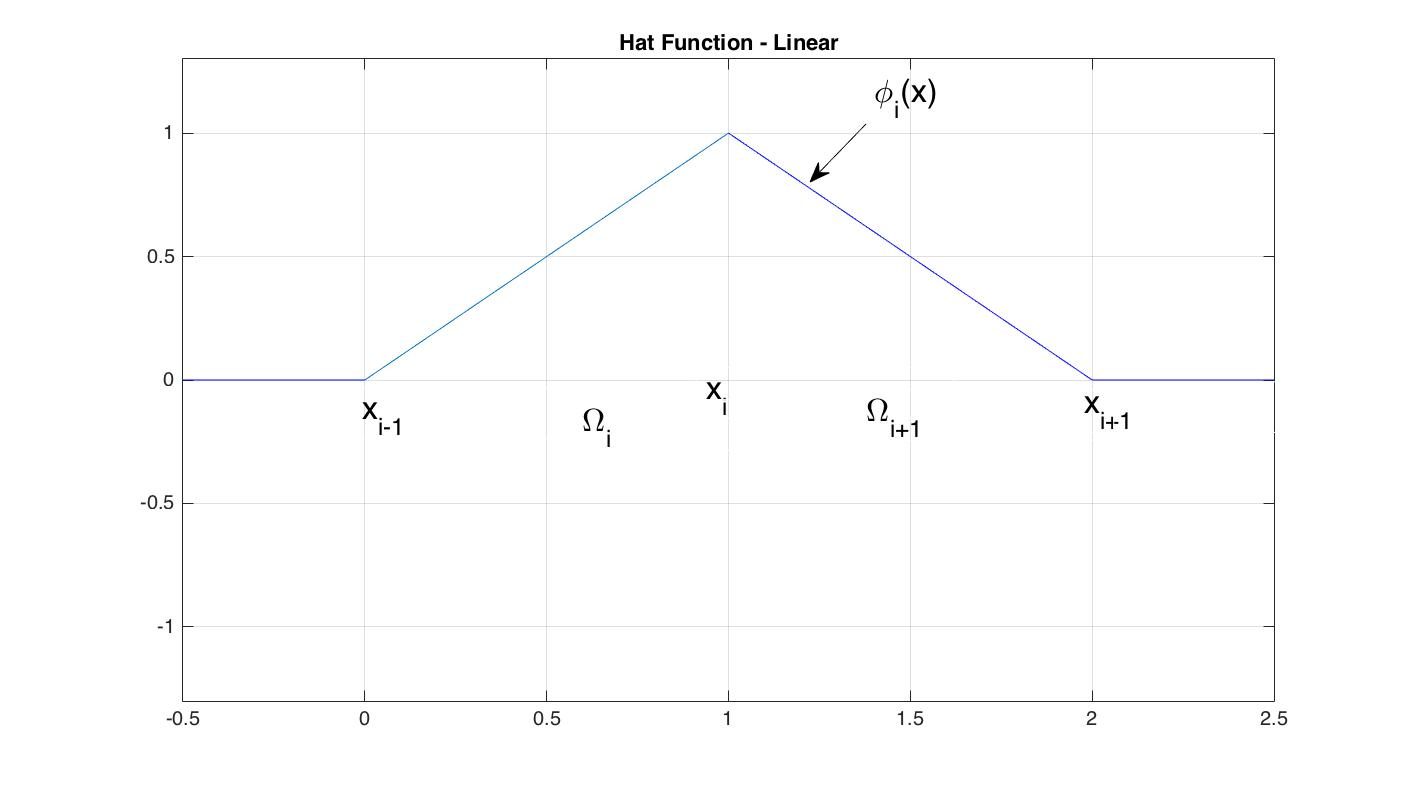
\includegraphics[width=12cm,height=8cm]{images/hat.jpg}
	\caption{Hat Function}
\end{figure}
\begin{equation}
\phi_i(x) = \left\{
\begin{array}{ll}
\frac{x-x_{i-1}}{h} & x_{i-1}\leq x\leq x_i \\
\frac{x_{i+1}-x}{h} & x_i\leq x\leq x_{i+1} \\
0 & otherwise\\
\end{array} 
\right. \label{basis1d}
\end{equation}
Observe that  
\begin{eqnarray}
\phi_i(x_j) &=& \delta_{ij}, \quad \text{where} \label{kd}\\
\delta_{ij} &=& \left\{ 
\begin{array}{ll}
1, & i=j\\
0, & i\ne j	
\end{array}
\right.
\end{eqnarray}
at nodes $x_j$. The expresssion \ref{basis1d} can be obtained by assuming a linear equation of the form $\phi_i(x) = a+b\ x$ and using the Kronecker Delta Property \ref{kd}. The function defined above is said to have a \textbf{Compact Support} in $\Omega$ which means that the function is non-zero only at certain points in the domain. This property is reflected in the \textbf{sparse nature} of the Global Stiffness Matrix.\\

To find out the solution at each nodes in the domain, we construct stiffness matrix $K^e$ and load vector $f^e$ at the element level and then assemble them to obtain the global system and solve it. So at the element level, we have the system of equations
\begin{eqnarray}
[K^e] \{u^e\} = \{f^e\}
\end{eqnarray}
The local numbering of the linear basis functions in an element $\Omega^e$ is shown in Figure 1.2(a). Let $\psi^e_1 \ \text{and} \ \psi^e_2$ be the basis function in an element $\Omega^e$. If the element size is $h_e$, then for the model problem in 1D, we have,
\begin{equation}
K^e = \Bigg[\int_{0}^{h_e} \psi_i'^e \psi_j'^e \ dx \Bigg]_{i,j=1,2} = 
\begin{bmatrix}
\frac{1}{h_e} & -\frac{1}{h_e} \\\\
-\frac{1}{h_e} & \frac{1}{h_e}
\end{bmatrix}
\end{equation}
\begin{center}
	\begin{figure}[h]
		\centering
		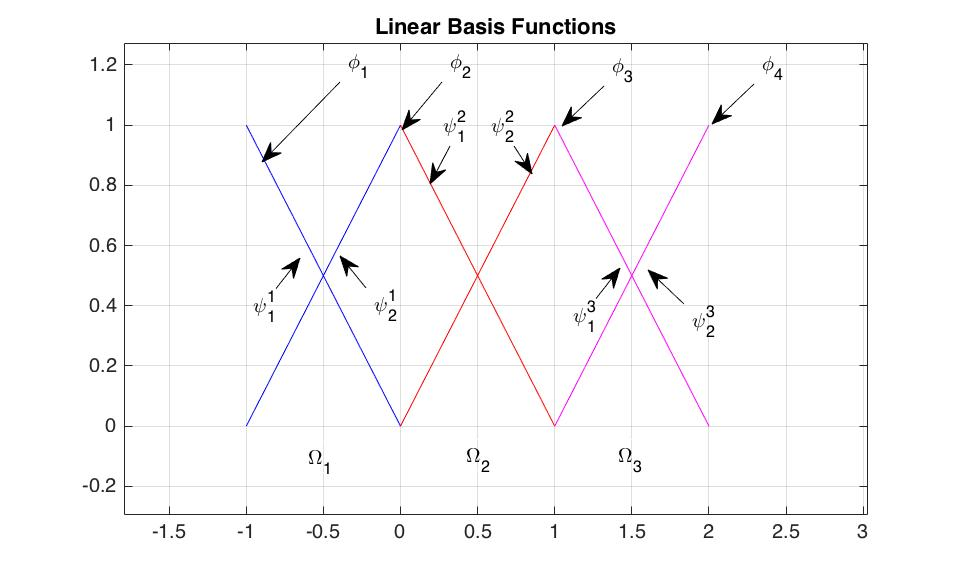
\includegraphics[scale = 0.4]{images/linearbasis.jpg}
		\caption{Basis Functions}
	\end{figure}
\end{center}
\pagebreak
\subsection{Assesmbly}
Upon adding the contributions of different element for any node $x_i$, we obtain the global stiffness matrix. This process is known as \textbf{Assembly} of the local siffness matrices. If $h_1, h_2, \dots, h_n$ are the element sizes, then the \textbf{global stiffness matrix A}  can easily be constructed as follows.
\begin{equation}
A = 
\begin{bmatrix}
\frac{1}{h_1} & -\frac{1}{h_1} & 0 & \dots & 0 & 0 & 0\\
-\frac{1}{h_1} & 	\frac{1}{h_1} + \frac{1}{h_2} & -\frac{1}{h_2} & \dots & 0 & 0 & 0\\
0 & 	-\frac{1}{h_2} & 	\frac{1}{h_2} + \frac{1}{h_3} & \dots & 0 & 0 & 0\\
\vdots & \vdots & \vdots & \vdots & \vdots & \vdots & \vdots\\
0 & 0 & 0 & \dots & -\frac{1}{h_{n-1}}  & \frac{1}{h_{n-1}} + \frac{1}{h_n} & 	-\frac{1}{h_n} \\
0 & 0 & 0 & \dots & 0  & -\frac{1}{h_n}  & \frac{1}{h_n} \\
\end{bmatrix} \label{assemA}
\end{equation}
and the \textbf{global load vector b} is,
\begin{equation}
b = 
\begin{Bmatrix}
\int_{0}^{h_1} f \psi_1^1 dx\\\\
\int_{0}^{h_1} f \psi_2^1 dx + \int_{h_1}^{h_2} f \psi_1^2 dx\\\\
\int_{h_1}^{h_2} f \psi_2^2 dx + \int_{h_2}^{h_3} f \psi_1^3 dx\\\\
\vdots\\\\
\int_{h_{n-2}}^{h_{n-1}} f \psi_2^{n-1} dx + \int_{h_{n-1}}^{h_n} f \psi_1^n dx\\\\
\int_{h_{n-1}}^{h_n} f \psi_2^n dx

\end{Bmatrix}\label{assemb}
\end{equation}
The next step is to apply the boundary conditions to the system $A \xi = b$ by setting the values accordingly in the Stiffness Matrix and Load Vector.\\


When we make the approximation by choosing $u_h$ from $V_h \subset V$, we introduce errors in the solution. If $u(x)$ denotes the exact solution and $u_h(x)$ denotes the Finite Element solution, we mention the following \textbf{error estimates} when a linear basis function is used. If $\lVert . \rVert_a$ denotes the energy norm, $\lVert . \rVert_\infty$ denotes the pointwise inifinity norm and $\lVert . \rVert_{H^m}$ denotes the $H^m$ norm we have the following error estimates
\begin{eqnarray}
\lVert u - u_h \rVert_a &\le& Ch \lVert u'' \rVert_\infty\\
\lVert u - u_h \rVert_{\infty} &\le& Ch^2 \lVert u'' \rVert_\infty \label{orderofconv}\\ 
\lVert u - u_h \rVert_{H^1} &\le& Ch \lVert u'' \rVert_\infty
\end{eqnarray}
Result \ref{orderofconv} shows that the Finite Element Method is second order accurate when linear basis is used.

\section{Numerical Examples}
\begin{example}
	Consider the following 2-Point Boundary Value Problem,
	\begin{eqnarray}
		-u'' = x(3+x)e^x, \quad 0<x<1\\
		u(0) = u(1) = 0
	\end{eqnarray}
	
		The exact solution is given by
		\begin{equation}
			u(x) = x(1-x)e^x
		\end{equation}
		
		We wish to find the solution to this problem using Finite Element Method.\\
		
		The weak form for the problem is given by \ref{weak1} with $f(x) = 1$ .\\
		
		 Assuming uniform grid spacing - $h$ while discretizing the domain into $n$ elements
		 \begin{eqnarray}
		 	 0&=&x_0 < x_2 < \dots < x_n = 1 \\
		 	 h &=& \frac{x_n - x_0}{n}\\
		 	 x_i &=& i \ h
		 \end{eqnarray}
		 
		  we have the finite dimensional weak form,
		 \begin{eqnarray}
		 	\text{Find} \; u_h \in V_h \subset V = H^1_0(0,1), \; \text{such that} \\
		 	\int_{0}^{1} u_h' v_h' \ dx = \int_{0}^{1} f v_h \ dx \quad \forall v_h \in V_h 	 	 
		 \end{eqnarray}	
		 
		 When we construct the element stiffness matrix, $K^e$, we get 
		 \begin{equation}
		 	K^e = \begin{bmatrix}
		 	\frac{1}{h} & -\frac{1}{h} \\
		 	-\frac{1}{h} & \frac{1}{h} 
		 	\end{bmatrix}
		 \end{equation}
		 
		 and after assembly (Ref. \ref{assemA}, \ref{assemb}) we obtain the system of linear equations.
		 \begin{equation}
		 	A \xi = b
		 \end{equation}
		 
		 and we solve the system of equations after accounting for the boundary conditions.	The solution plots for different number of elements are shown in Figure,\\
		 
		 \begin{figure}[h!]
		 		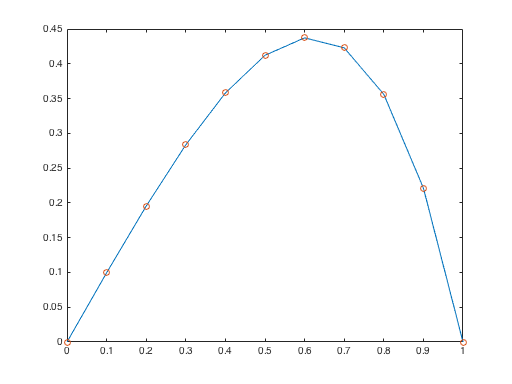
\includegraphics[scale = 0.8]{images/firstex.png}
		 		\caption{$Numerical Solution$}
		 \end{figure}
		 
		The infinity norm of the error in the Finite Element Solution was found out to be in the order of $\approx 10^{-16}$ which is very close to the machine error $\approx 2.2 \times 10^{-16}$
		

\end{example}

\begin{example}
		Consider the following 2-Point Boundary Value Problem,
		\begin{eqnarray}
		-u'' + u &=& 12x + 3x^2 - 2x^3 - 6, \quad 0<x<1\\
		u(0) &=& 0\\
		u'(1) &=& 0
		\end{eqnarray}
		
		The weak form for this problem is given by,
		\begin{eqnarray}\nonumber
		\text{Find} \; u_h \in V_h \subset V = \{u \ | \ u \in H^1(0,1), \ u(0) = 0\}, \; \text{such that} \\\nonumber
		- u_h'v_h \Big|_0^1 + \int_{0}^{1} (u_h' v_h' + u_h v_h) \ dx = \int_{0}^{1} f v_h \ dx \qquad &\forall v_h \in V_h&	\\
		\implies \int_{0}^{1} (u_h' v_h' + u_h v_h) \ dx = \int_{0}^{1} f v_h \ dx  + u_h'(1)v_h(1)\qquad &\forall v_h \in V_h&\\
		\implies \int_{0}^{1} (u_h' v_h' + u_h v_h) \ dx = \int_{0}^{1} f v_h \ dx  \qquad &\forall v_h \in V_h&
		\end{eqnarray}	
		
		The Neumann Boundary Condition is accounted in the assembled RHS by adding the value of $u'(1)$ in the last entry of $b$.\\
		
		Hence the final system of equations become,
		\begin{equation}
			A \xi = b + \vec{f_n}
		\end{equation}
		
The order of convergence observed for different elements are tabulated below,\\
		\begin{center}
			\begin{tabular}{|c|c|}
				\hline
				Element Type & Order of convergence observed\\
				\hline
				Linear & $\approx 2$\\
				Quadratic & $\approx 4$\\
				Cubic & $\approx 5$\\
				\hline						
			\end{tabular}
		\end{center}
		\begin{figure}[h!]
						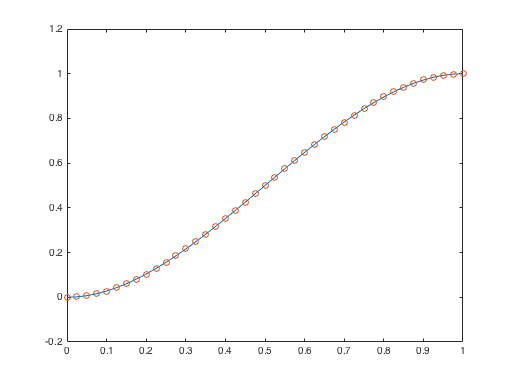
\includegraphics[scale = 0.8]{images/secondex.png}
						\caption{$n = 40$}	
		\end{figure}
\end{example}

\begin{example}
	Consider the following 2-Point Boundary Value Problem,
	\begin{eqnarray}
	-u'' + u &=& x^2+x-2, \quad 0<x<1\\
	u(0) &=& 0\\
	u(1)+u'(1) &=& 5
	\end{eqnarray}
	
	The weak form for this problem is given by,
	\begin{eqnarray}\nonumber
	\text{Find} \; u_h \in V_h \subset V = \{u \ | \ u \in H^1(0,1), \ u(0) = 0\}, \; \text{such that} \\\nonumber
	- u_h'v_h \Big|_0^1 + \int_{0}^{1} (u_h' v_h' + u_h v_h) \ dx = \int_{0}^{1} f v_h \ dx \qquad &\forall v_h \in V_h&	\\
	\implies \int_{0}^{1} (u_h' v_h' + u_h v_h) \ dx = \int_{0}^{1} f v_h \ dx  + u_h'(1)v_h(1)\qquad &\forall v_h \in V_h&\\
	\implies \int_{0}^{1} (u_h' v_h' + u_h v_h) \ dx = \int_{0}^{1} f v_h \ dx  + (5 - u_h(1)) \ v_h(1)\qquad &\forall v_h \in V_h&
	\end{eqnarray}	
	The Robin Boundary Condition is accounted in the assembled R.H.S by adding the value of $u'(1)+u(1) = 5$ in the last entry of $b$, and since $u_h(1)$ appears in the R.H.S, the value must be accounted for in the assembled global stiffness matrix.\\
	
	Hence the final system of equations become,
	\begin{equation}
		\begin{bmatrix}
		A_{11} & A_{12} & \dots & A_{1n}\\
		\vdots & \vdots & \vdots & \vdots\\
		A_{n1} & A_{n2} & \dots & A_{nn}
		\end{bmatrix} 
		\begin{Bmatrix}
		\xi_1\\
		\vdots\\
		\xi_n
		\end{Bmatrix} = 
		\begin{Bmatrix}
		b_1\\
		\vdots\\
		b_n
		\end{Bmatrix} +
		\begin{Bmatrix}
		0\\
		\vdots\\
		5 - \xi_n
		\end{Bmatrix}
	\end{equation}
	which in-turn becomes,
	\begin{equation}
		\begin{bmatrix}
		A_{11} & A_{12} & \dots & A_{1n}\\
		\vdots & \vdots & \vdots & \vdots\\
		A_{n1} & A_{n2} & \dots & A_{nn}+1
		\end{bmatrix} 
		\begin{Bmatrix}
		\xi_1\\
		\vdots\\
		\xi_n
		\end{Bmatrix} = 
		\begin{Bmatrix}
		b_1\\
		\vdots\\
		b_n
		\end{Bmatrix} +
		\begin{Bmatrix}
		0\\
		\vdots\\
		5
		\end{Bmatrix}
	\end{equation}
	
	The plots showing the solution curves for a Cubic Element is shown in Figure \ref{fig5}. The error in the Finite Element solution is in the order of $\approx 10^{-13}$
	
	\begin{figure}[h!]
			\begin{subfigure}{0.5\textwidth}
				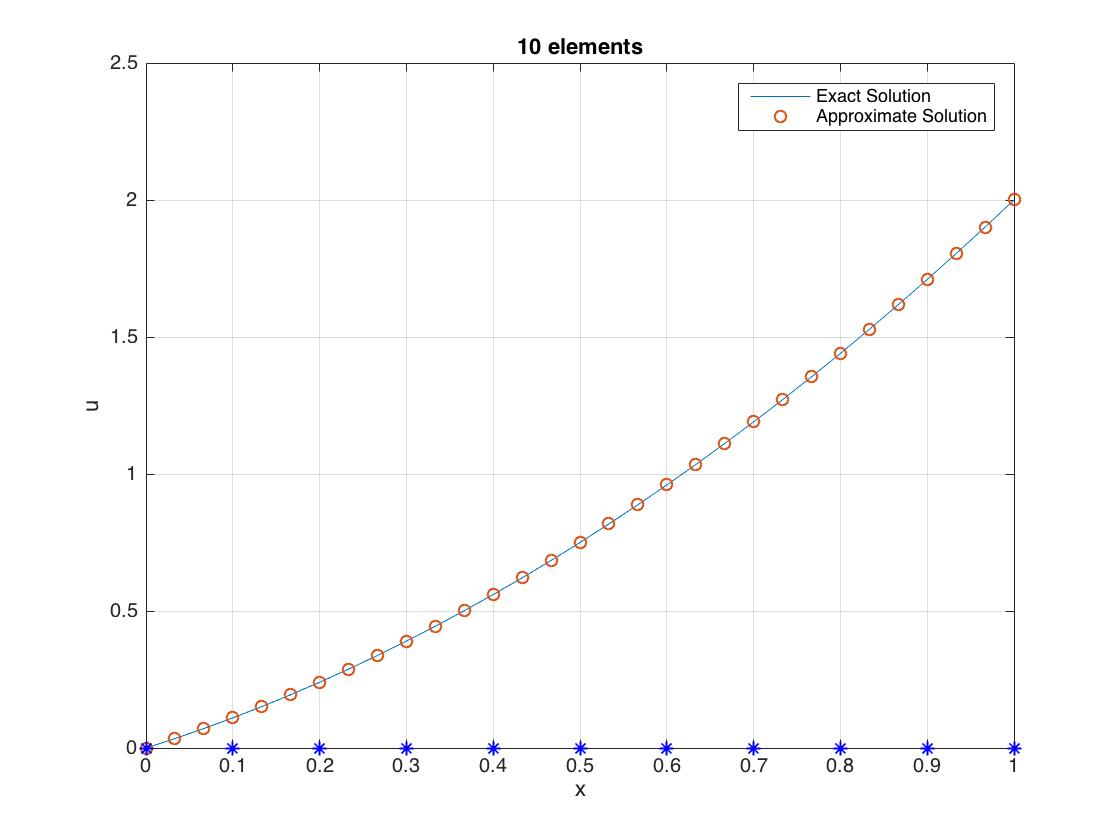
\includegraphics[scale = 0.2]{images/ex3/cubic10.jpg}
				\caption{$n = 10$}	
			\end{subfigure}
			\begin{subfigure}{0.5\textwidth}
				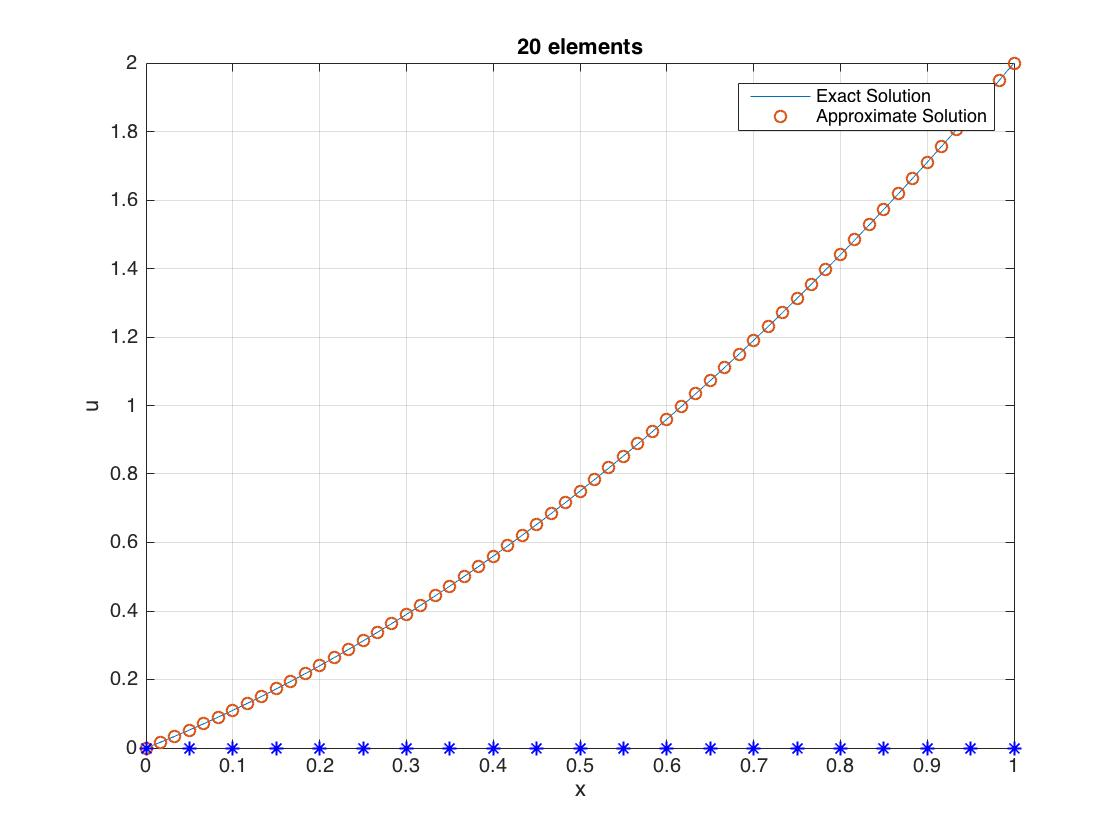
\includegraphics[scale = 0.2]{images/ex3/cubic.jpg}
				\caption{$n = 20$}	
			\end{subfigure}
			\caption{Solution plots using cubic elements - Example 2.3}
			\label{fig5}		
	\end{figure}
\end{example}

\section{Non-Linear Problem}
Next we consider solving a non-linear problem using Finite Element Method. We obtain a non-linear system of equations,
\begin{equation}
	K(U) \ U = F \quad \text{or} \quad K U = F(U) 
\end{equation}
So, we use the \textbf{Newton Raphson} iterations to solve the system of equations. The procedure is to first construct the system of equations at the element level,
\begin{equation}
	K^e(u^e) \ u^e = f^e
\end{equation}
and compute the elemental Jacobian Matrix $J^e$. Next we assemble the elemental Jacobian and the elemental load vector to the global level $J$ and $F$ and use Newton Raphson Iterations,
\begin{enumerate}
	\item Define $error = 100$ and tolerance $tol = 10^{-10}$ and Initial Guess $U_{old}$.
	\item Compute elemental Jacobian Matrix and Load Vector $J^e$ and $F^e$
	\item while $error > tol$:
	\begin{eqnarray}\nonumber
		&\text{Assemble: }& \quad J^e \ \text{and} \ F^e \implies J \ and \ F\\\nonumber
		&\text{Apply Boundary Conditions}&\\\nonumber
		& \text{Newton Raphson Iteration:}& \quad U_{new} = U_{old} - (J^{-1} F)(U_{old})\\\nonumber
		& \text{Set} & \quad error = \lVert U_{new} - U_{old} \rVert\\\nonumber
		& \text{Do} & \quad U_{old} = U_{new}
	\end{eqnarray}
\end{enumerate}

\begin{example}
	Consider the following 2-Point Boundary Value Problem,
	\begin{eqnarray}
	-u'' + (u')^3 &=& 0, \quad 0<x<1\\
	(u+u')(0) &=& 3/\sqrt{2}\\
	u'(1) &=& 0.5
	\end{eqnarray}
	
	The exact and the approximate solution are shown in Figure \ref{fig6}. The order of convergence is found to be $2$, when linear basis functions are used.
	\begin{figure}[h]
		\begin{subfigure}{0.5\textwidth}
			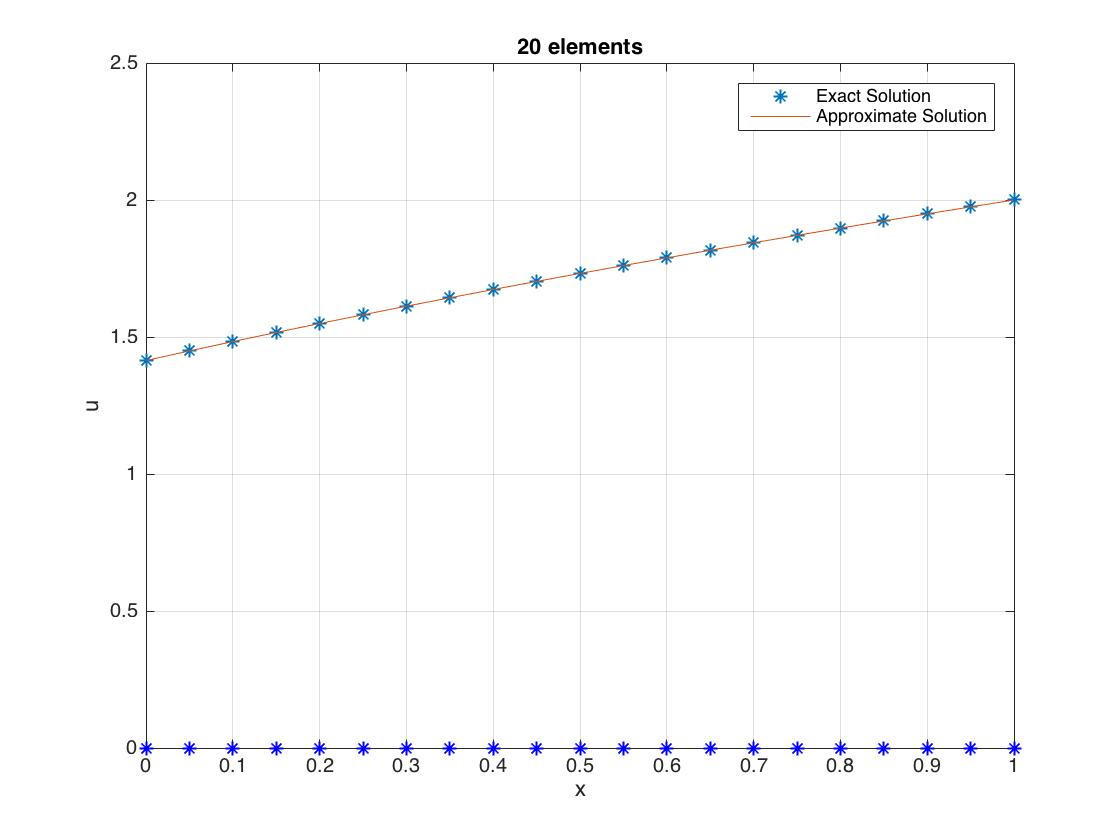
\includegraphics[scale = 0.2]{images/ex4/nonlinear.jpg}
			\caption{$n=20$}
		\end{subfigure}	
	\begin{subfigure}{0.5\textwidth}
		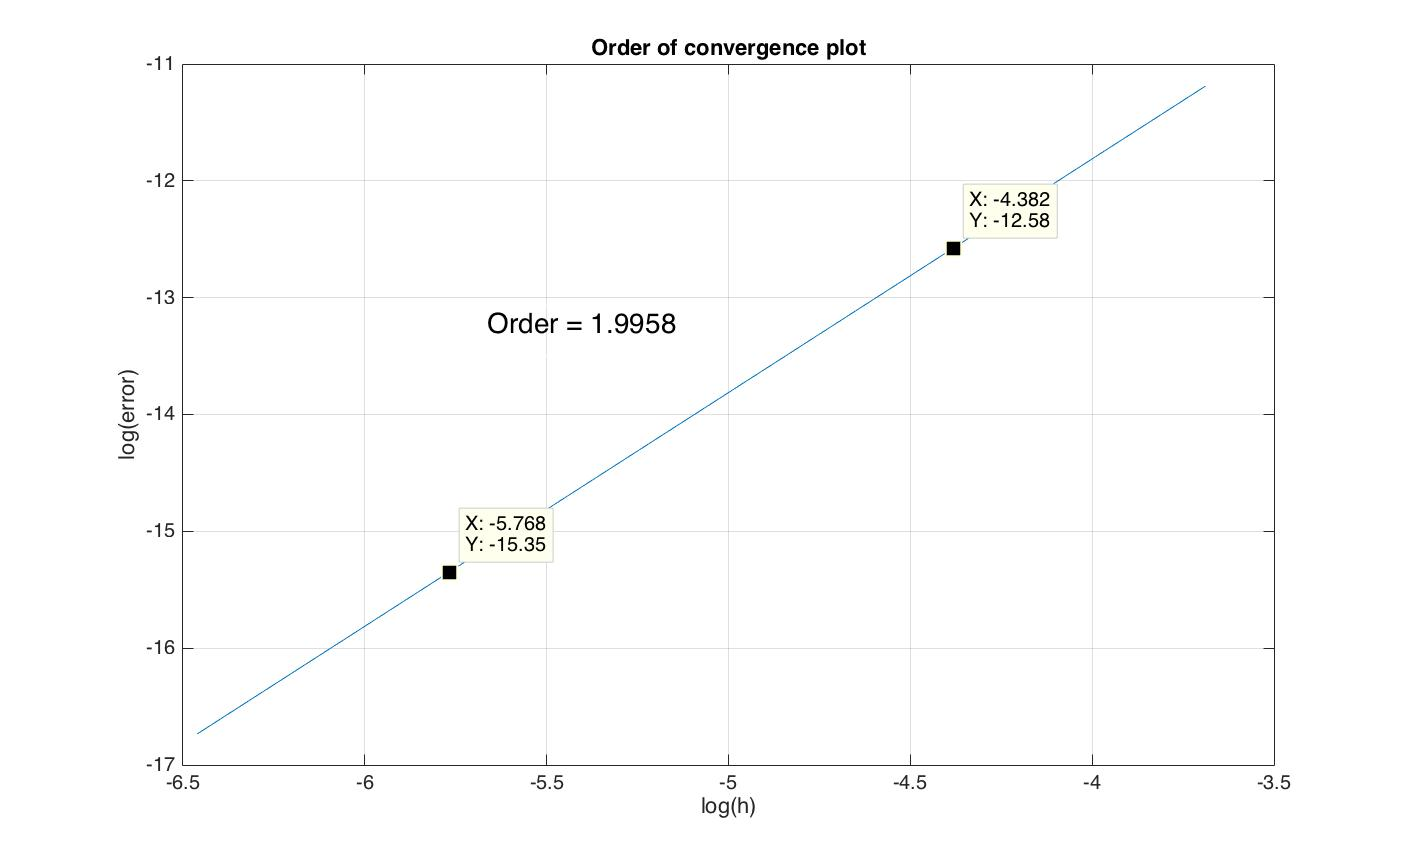
\includegraphics[scale = 0.2]{images/ex4/non_order.jpg}
		\caption{Order of convergence $\approx 2$}
	\end{subfigure}
	\caption{Non Linear Problem - Example 2.4}	
	\label{fig6}
	\end{figure}
\end{example}

	
	\chapter{2D Elliptic problems in FEniCS}
	% Report/chapters/ff.tex

The FEniCS Project is a collaborative project for the development of innovative concepts and tools for automated scientific computing, with a particular focus on automated solution of differential equations by finite element methods. 
FEniCS has an extensive list of features for automated, efficient solution of differential equations, including automated solution of variational problems, automated error control and adaptivity, a comprehensive library of finite elements, high performance linear algebra and many more.

\smallskip
\noindent This chapter discusses how to solve a Boundary Value Problem, in particular 2D problems using FreeFEM++.

\section{Model Problem}
Consider the following model problem,
\begin{eqnarray}
	-\Delta u &=& f, \quad \text{in} \ \Omega \\
	u &=& z \quad \text{on} \ \Gamma_1\\
	\frac{\partial u}{\partial n}  &=& \nabla u . n = 0 \quad \text{on} \ \Gamma_2
\end{eqnarray}

The FEniCS code that solves the problem is given below.

\lstset{language = python}
\begin{lstlisting}
	-Laplace(u) = f on the unit square.
	u = u0 on the boundary.
	u0 = u = 1 + x^2 + 2y^2, f = -6.
	
	from dolfin import *
	mesh = UnitSquare(6, 4)
	V = FunctionSpace(mesh, 'Lagrange', 1)
	
	u0 = Expression('1 + x[0]*x[0] + 2*x[1]*x[1]')
	
	def u0_boundary(x, on_boundary):
	return on_boundary
	
	bc = DirichletBC(V, u0, u0_boundary)
	
	u = TrialFunction(V)
	v = TestFunction(V)
	f = Constant(-6.0)
	a = inner(nabla_grad(u), nabla_grad(v))*dx
	L = f*v*dx
	
	u = Function(V)
	solve(a == L, u, bc)
	
	plot(u)
	plot(mesh)
	
	interactive()
\end{lstlisting}

Let us first look at some important commands and syntax that are necessary to understand further problems.
\begin{lstlisting}
	from dolfin import *
\end{lstlisting}
This line imports the key classes UnitSquare, FunctionSpace, Function, and so forth, from the DOLFIN library. All FEniCS programs for solving PDEs by the finite element method normally start with this line. DOLFIN is a software library with efficient and convenient C++ classes for finite element computing, and dolfin is a Python package providing access to this C++ library from Python programs.

\begin{lstlisting}
	mesh = UnitSquare(6, 4)
\end{lstlisting}
The UnitSquare command defines a uniform finite element mesh over the unit square. The mesh consists of cells, which are triangles with straight sides. The parameters 6 and 4 tell that the square is first divided into 6×4 rectangles, and then each rectangle is divided into two triangles.
Other types of mesh generation will be discussed in the later part of this chapter.
\begin{lstlisting}
	V = FunctionSpace(mesh, 'Lagrange', 1)
\end{lstlisting}
The functionspace command defines a function space V with 3 arguments. The first argument is the mesh. The second argument reflects the type of element, while the third argument is the degree of the basis functions on the element.

\begin{figure}[h]
	\center
	
\includegraphics[scale = 0.25]{images/mesh.png}
	\caption{FEniCS Mesh}
\end{figure}

\begin{lstlisting}
	u = TrialFunction(V)
	v = TestFunction(V)
\end{lstlisting}
These commands define the finite dimensional trial and test spaces.
\begin{lstlisting}
	bc = DirichletBC(V, u0, u0_boundary)
\end{lstlisting}
The next step is to specify the boundary condition on the boundary.
\begin{lstlisting}
	f = Constant(-6.0)
\end{lstlisting}
When \textbf{f} is constant over the domain, \textbf{f} can be more efficiently represented as a Constant object.

We input the weak form of the problem 
\begin{eqnarray}
	 \int_{\Omega} \nabla u_h. \nabla v_h \ d\Omega - \int_{\Omega} f v_h \ d\Omega = 0
\end{eqnarray}
with the boundary condtions. The \textbf{solve} command solves the problem yielding $u_h$. 
\begin{lstlisting}
	a = inner(nabla_grad(u), nabla_grad(v))*dx
	L = f*v*dx
	u = Function(V)
	solve(a == L, u, bc)
\end{lstlisting}
Note that we first defined the variable $u$ as a TrialFunction and used it to represent the unknown in the form $a$. Thereafter, we redefined $u$ to be a Function object representing the solution, i.e., the computed finite element function $u$.
\begin{lstlisting}
	plot(u)
	plot(mesh)
	interactive()
\end{lstlisting}
This is the simplest way of quickly looking at $u$ and the mesh. The interactive() call is necessary for the plot to remain on the screen.

\pagebreak

\section{Meshing in Fenics}
In this section we will discuss a couple of standard mesh generation techniques.
\subsection{Built-in Mesh generation tools}
DOLFIN has a few tools for creating various types of meshes over domains with simple shape: \textbf{UnitInterval, UnitSquare, UnitCube, Interval, Rectangle, Box, UnitCircle, and UnitSphere}.
\begin{lstlisting}
	# 1D domains
	mesh = UnitInterval(20)     # 20 cells, 21 vertices
	mesh = Interval(20, -1, 1)  # domain [-1,1]

	# 2D domains (6x10 divisions, 120 cells, 77 vertices)
	mesh = UnitSquare(6, 10)  # 'right' diagonal is default
	# The diagonals can be right, left or crossed
	mesh = UnitSquare(6, 10, 'left')
	mesh = UnitSquare(6, 10, 'crossed')

	# Domain [0,3]x[0,2] with 6x10 divisions and left diagonals
	mesh = Rectangle(0, 0, 3, 2, 6, 10, 'left')

	# 6x10x5 boxes in the unit cube, each box gets 6 tetrahedra:
	mesh = UnitCube(6, 10, 5)

	# Domain [-1,1]x[-1,0]x[-1,2] with 6x10x5 divisions
	mesh = Box(-1, -1, -1, 1, 0, 2, 6, 10, 5)

	# 10 divisions in radial directions
	mesh = UnitCircle(10)
	mesh = UnitSphere(10)
\end{lstlisting}

\subsection{Other techniques}

Other standard techniques for importing/generating meshes into FEniCS are reading \textbf{.XML or .OFF} files, using the Mesheditor, using a few \textbf{CGAL} functions or using \textbf{dolfin-convert}.

\noindent XML and OFF files are formats which are useful for saving and communicating meshes, not for generating them. \textbf{CGAL} stands for Computational Geometry Algorithms Library. Some of the few commands in \textbf{CGAL} are \textbf{CircleMesh, EllipseMesh, SphereMesh, EllipsoidMesh, PolyhedralMeshGenerator, Add ,Subtract }etc

\pagebreak

\section{Linear Numerical examples}

\begin{lstlisting}
	-Laplace(u) = f on the unit square.
	u = u0 on the boundary.
	u0 = 1 + x^2 + 2y^2, f = -6.
\end{lstlisting}
\begin{figure}[h]
	\center
	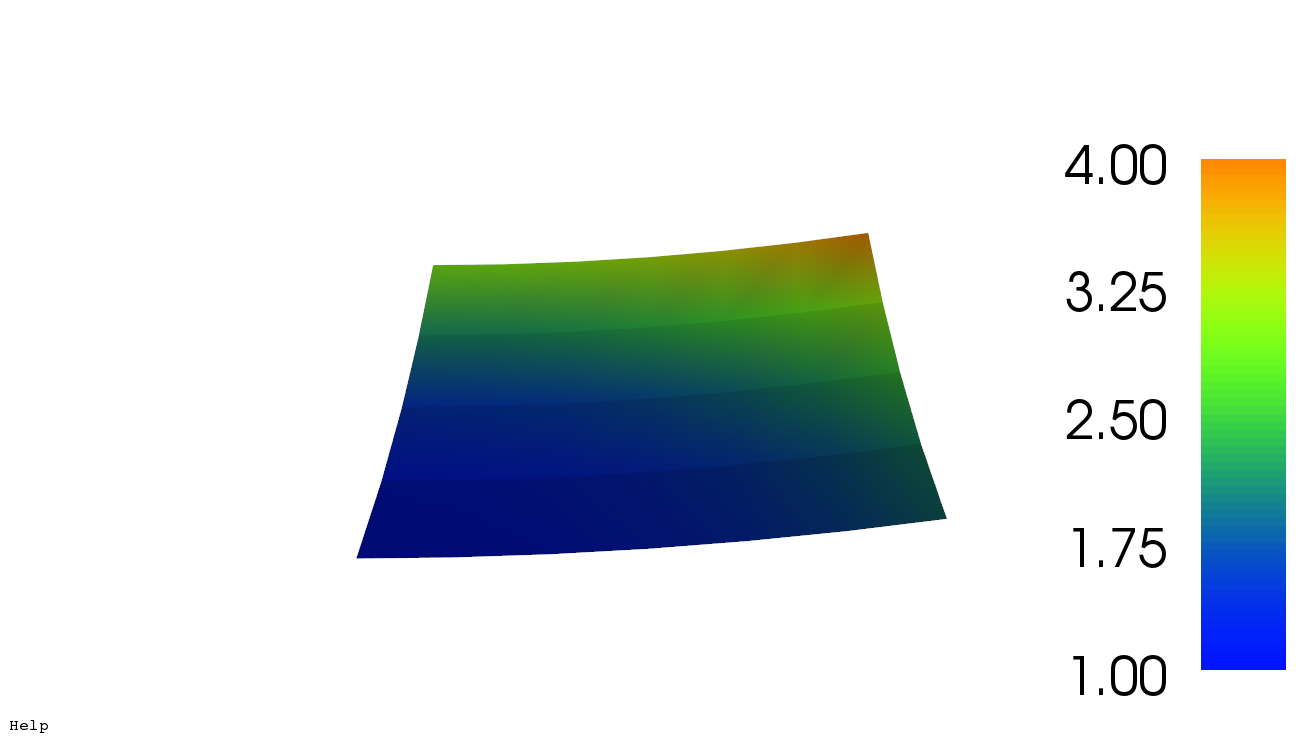
\includegraphics[scale = 0.25]{images/dirichlet.png}
	\caption{FEniCS Solution}
\end{figure}

Order of convergence data for Linear largrange element
\begin{lstlisting}
	Error norm based on infinity norm (of dofs)
	h=1.25E-01 E=3.75E-02 r=1.88
	h=6.25E-02 E=9.57E-03 r=1.97
	h=3.12E-02 E=2.41E-03 r=1.99
	h=1.56E-02 E=6.02E-04 r=2.00
	h=7.81E-03 E=1.51E-04 r=2.00
	h=3.79E-03 E=3.54E-05 r=2.00
\end{lstlisting}
\pagebreak
\noindent \textbf{Dirichlet Neumann Problem}
\begin{lstlisting}
	- div grad u(x, y) = f(x, y)
	on the unit square with source f given by
	f(x, y) = 10*exp(-((x - 0.5)^2 + (y - 0.5)^2) / 0.02)
	and boundary conditions given by
	u(x, y) = 0        for x = 0 or x = 1
	du/dn(x, y) = sin(5*x) for y = 0 or y = 1
\end{lstlisting}
\begin{figure}[h]
	\center
	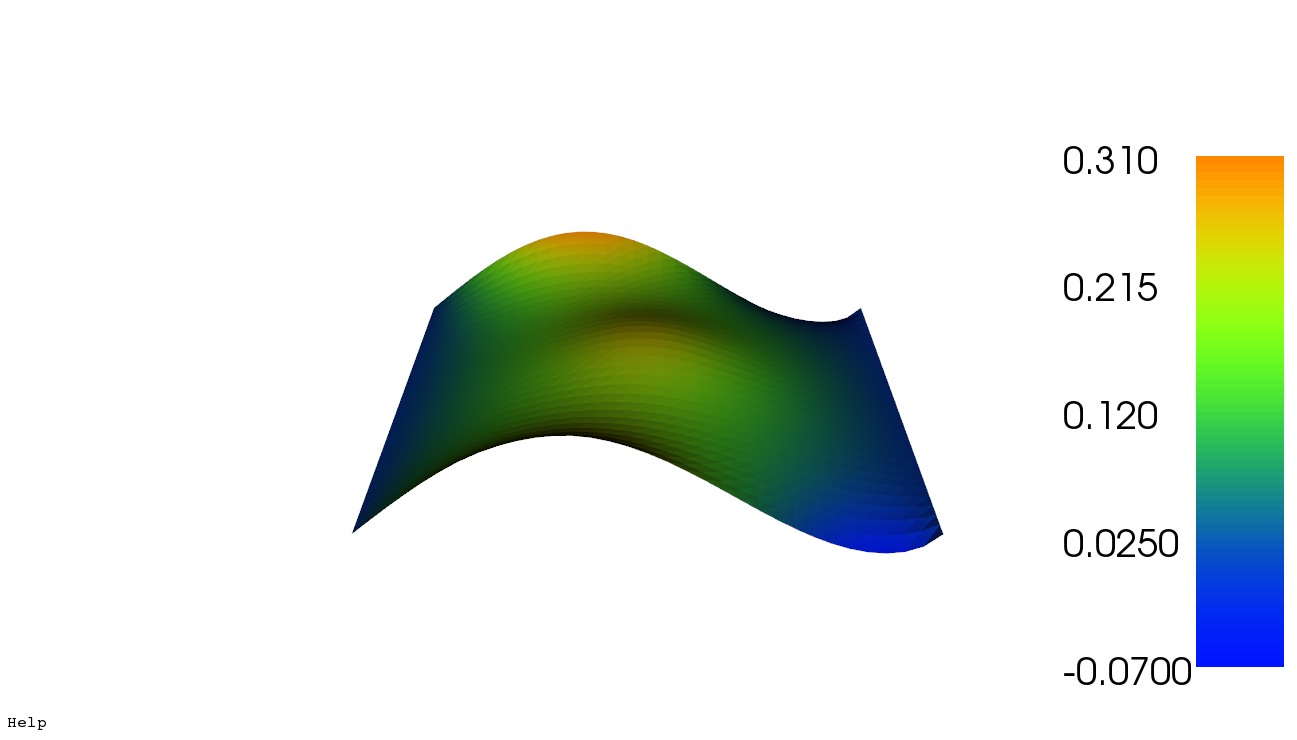
\includegraphics[scale = 0.25]{images/dn.png}
	\caption{FEniCS Solution}
\end{figure}
\noindent The order of convergence data for cubic Lagrange element
\begin{lstlisting}
	Error norm based on infinity norm (of dofs)
	h=5.00E-02 E=7.36E-06 r=3.97588
	h=2.50E-02 E=4.62E-07 r=3.99406
	h=1.25E-02 E=2.89E-08 r=3.99884
	h=6.25E-03 E=1.78E-09 r=4.01965
\end{lstlisting}

\pagebreak
\section{Nonlinear Problems}
Now we shall address how to solve nonlinear PDEs in FEniCS. Our sample PDE for implementation is taken as a nonlinear Poisson equation:
\begin{equation}
-\nabla\cdot\left( q(u)\nabla u\right) = f\thinspace .
\end{equation}
The coefficient $q(u)$ makes the equation nonlinear (unless $q(u)$ is constant in $u$).

\noindent The variational formulation of our model problem reads: Find $u\in V$ such that
\begin{equation}
F(u; v) = 0 \quad \forall v \in \hat{V},
\end{equation}
where
\begin{equation}
F(u; v) = \int_\Omega q(u)\nabla u\cdot \nabla v \, \mathrm{d}x,
\end{equation}
and
\begin{eqnarray}
\begin{split}\hat{V} &= \{v \in H^1(\Omega) : v = 0 \mbox{ on } x_0=0\mbox{ and }x_0=1\}, \\
V      &= \{v \in H^1(\Omega) : v = 0 \mbox{ on } x_0=0\mbox{ and } v = 1\mbox{ on }x_0=1\}\thinspace .\end{split}
\end{eqnarray}
The discrete problem arises as usual by restricting $V$ and $\hat{V}$ to a pair of discrete spaces. The discrete nonlinear problem is then wirtten as: find $u\in V$ such that
\begin{equation}
F(u; v) = 0 \quad \forall v \in \hat{V},
\end{equation}

\subsection{Picard Iteration}
Picard iteration is an easy way of handling nonlinear PDEs: we simply use a known, previous solution in the nonlinear terms so that these terms become linear in the unknown $u$. The strategy is also known as the method of successive substitutions. For our particular problem, we use a known, previous solution in the coefficient $q(u)$. More precisely, given a solution $u_k$ from iteration $k$, we seek a new (hopefully improved) solution $u_{k+1}$ in iteration $k+1$ such that $u_{k+1}$ solves the linear problem,
\begin{equation}
\nabla\cdot \left(q(u^k)\nabla u^{k+1}\right) = 0,\quad k=0,1,\ldots
\end{equation}
The iterations require an initial guess $u^0$. The hope is that $uk\rightarrow u$ as $k \rightarrow \infty$, and that $u^{k+1}$ is sufficiently close to the exact solution $u$ of the discrete problem after just a few iterations.

\pagebreak
\subsection{Newton Method at the Algebraic Level}
After having discretized our nonlinear PDE problem, we may use Newton’s method to solve the system of nonlinear algebraic equations. From the continuous variational problem, the discrete version results in a system of equations for the unknown parameters $U_1,…,U_N$.

\smallskip

\noindent In order to calculate the solution FEniCS has an inbuilt function to carry out Jacobian calculation and finally solving it by Newton Raphson iteration.

\smallskip

\noindent Note the important feature in Newton’s method that the previous solution $u_k$ replaces $u$ in the formulas when computing the matrix $\partial F_i/\partial U_j$ and vector $F_i$ for the linear system in each Newton iteration.

\pagebreak

	
	\chapter{Time Dependent Problems in FEniCS}
	%parabolic
Many researchers will prefer to code the solution strategy of the nonlinear problem themselves and experiment with various combinations of strategies in difficult problems. Time-dependent problems are somewhat similar in this respect: we have to add a time discretization scheme, which is often quite simple, making it natural to explicitly code the details of the scheme so that the programmer has full control. We shall explain how easily this is accomplished through examples.

\section{Diffusion Problem and its Discretization}
Let our problem be defined as,
\begin{eqnarray}
\begin{split}{\partial u\over\partial t} &= \nabla^2 u + f \mbox{ in } \Omega, \hbox{ for } t>0,
\\
u &= u_0 \mbox{ on } \partial \Omega,\hbox{ for } t>0,
\\
u &= I   \mbox{ at } t=0\thinspace .\end{split}
\end{eqnarray}
Here, $u$ varies with space and time, e.g., $u=u(x,y,t)$ if the spatial domain $\Omega$ is two-dimensional. The source function $f$ and the boundary values $u0$ may also vary with space and time. The initial condition $I$ is a function of space only.

\noindent The time-derivative can be approximated by a finite difference. For simplicity and stability reasons we choose a simple backward difference:
\begin{eqnarray}
{\partial \over\partial t}u^k\approx {u^k - u^{k-1}\over{\Delta t}},
\end{eqnarray}
where $\Delta t$ is the time discretization parameter.

\pagebreak

Inserting this approximation in the PDE yields
\begin{equation}
{{u^k - u^{k-1}\over{\Delta t}} = \nabla^2 u^k + f^k\thinspace .}
\end{equation}
We use a finite element method to solve the time-discrete equations which still have spatial differential operators. This requires turning the equations into weak forms. As usual, we multiply by a test function $v\in V̂$ and integrate second-derivatives by parts. Introducing the symbol $u$ for $u^k$ , the resulting weak form can be conveniently written in the standard notation: $a_0(u,v)=L_0(v)$ for the initial step and $a(u,v)=L(v)$ for a general step, where
\begin{eqnarray}
\begin{split}a_0(u,v) &= \int_\Omega uv \, \mathrm{d}x, \\
L_0(v) &= \int_\Omega Iv \, \mathrm{d}x, \\
a(u,v) &= \int_\Omega\left( uv + {\Delta t}
\nabla u\cdot \nabla v\right) \, \mathrm{d}x, \\
L(v) &= \int_\Omega \left(u^{k-1} + {\Delta t}  f^k\right)v \, \mathrm{d}x\thinspace .\end{split}
\end{eqnarray}
The continuous variational problem is to find $u^0\in V$ such that $a_0(u^0,v)=L_0(v)$ holds for all $v\in \hat{V}$ , and then find $u^k\in V$ such that $a(u^k,v)=L(v)$ for all $v\in\hat{V}$, $k=1,2,…$
\pagebreak
\section{Numerical Example}
\begin{lstlisting}
	du/dt -Laplace(u) = f on the unit square.
	u = u0 on the boundary.
	u = I at t=0
\end{lstlisting}
\begin{figure}[h]
	\center
	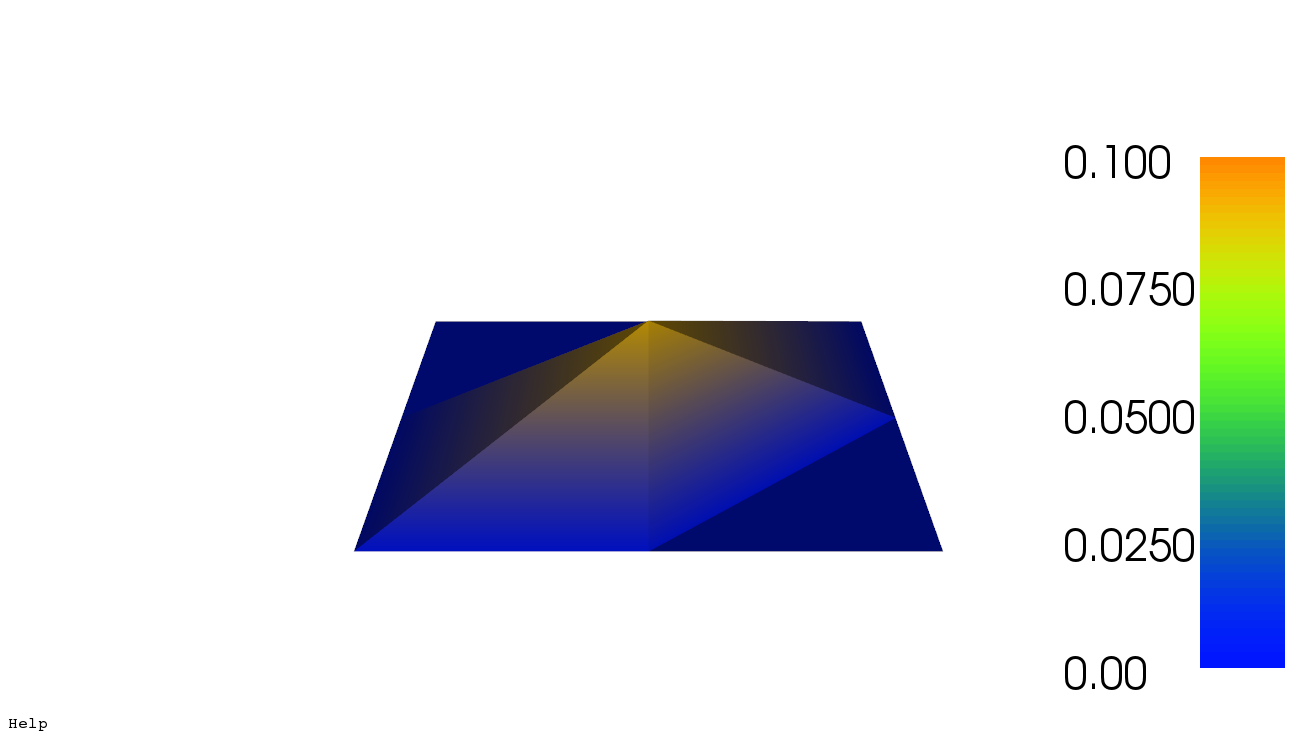
\includegraphics[scale = 0.25]{images/4.png}
	\caption{$2 * 2$ elements}
\end{figure}
Order of convergence data
\begin{lstlisting}
Max error in Run 1 is 0.05900472985458862785
Max error in Run 2 is 0.02119882894487590264
Max error in Run 3 is 0.00550957587228301238
Max error in Run 4 is 0.00110141248956971416
Max error in Run 5 is 0.00005668741721423509
Order of convergence
1.47684603606
1.94397140098
2.32258639099
4.2801825243
\end{lstlisting}
\begin{figure}[h]
	\center
	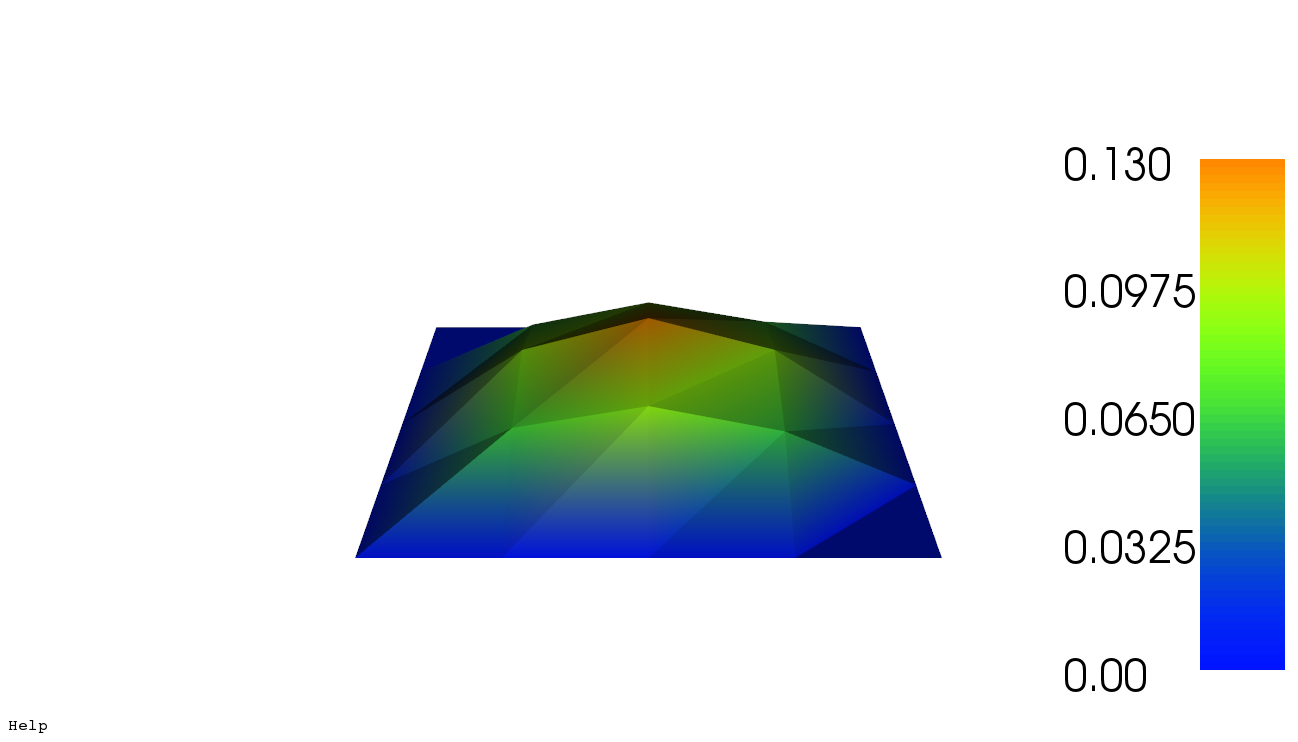
\includegraphics[scale = 0.25]{images/16.png}
	\caption{$4 * 4$ elements}
\end{figure}
\begin{figure}[h]
	\center
	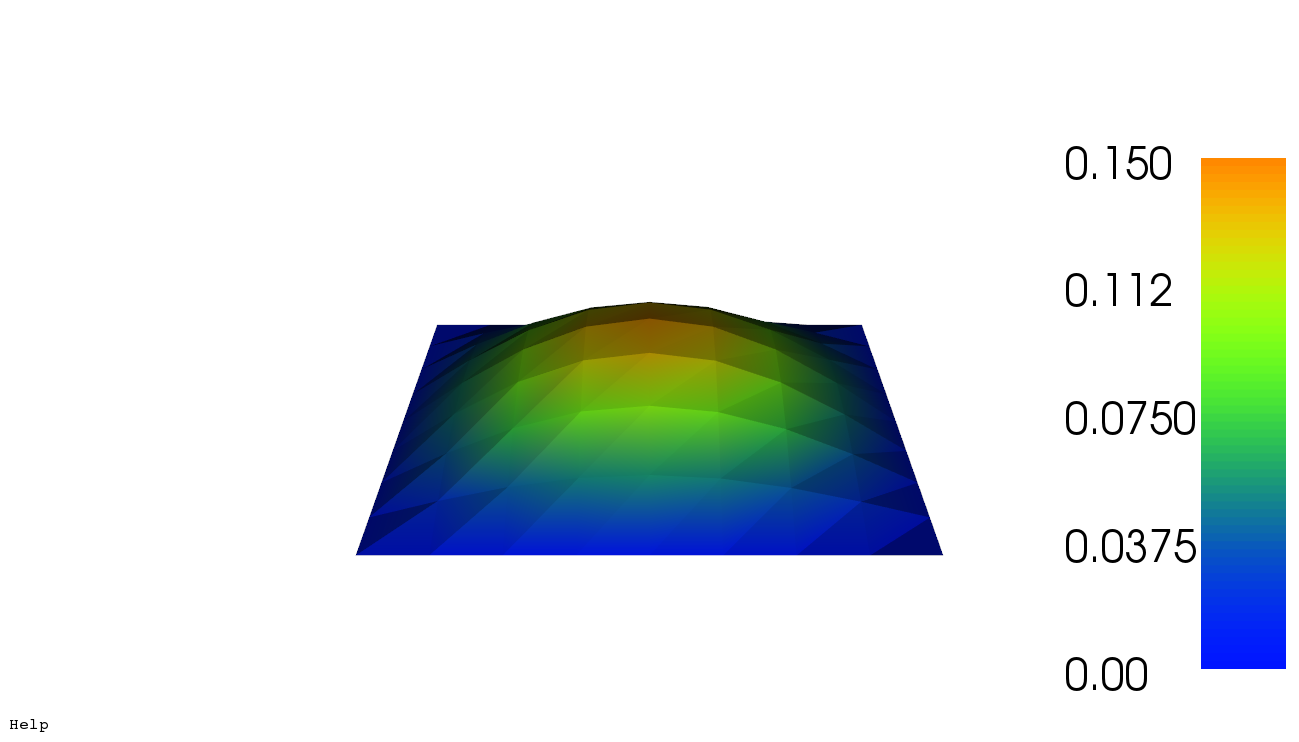
\includegraphics[scale = 0.25]{images/64.png}
	\caption{$8 * 8$ elements}
\end{figure}
\begin{figure}[h]
	\center
	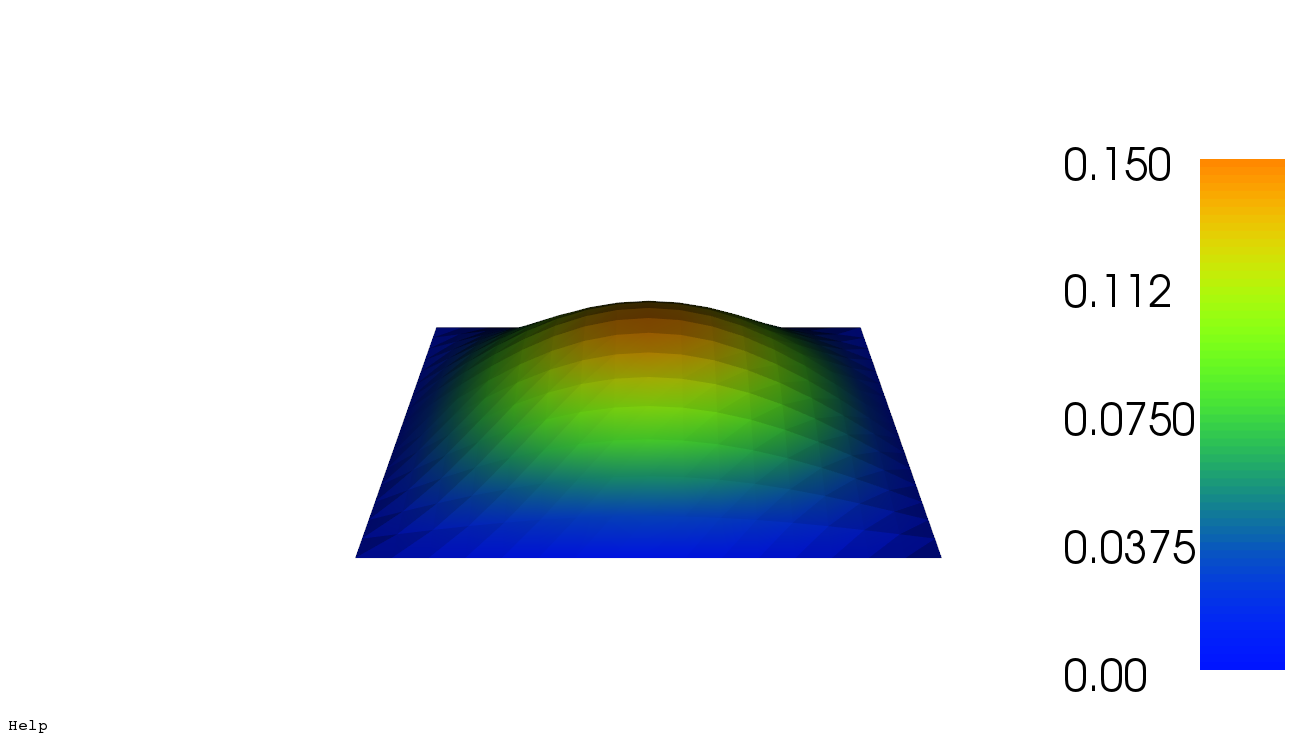
\includegraphics[scale = 0.25]{images/256.png}
	\caption{$16 * 16$ elements}
\end{figure}
\begin{figure}[h]
	\center
	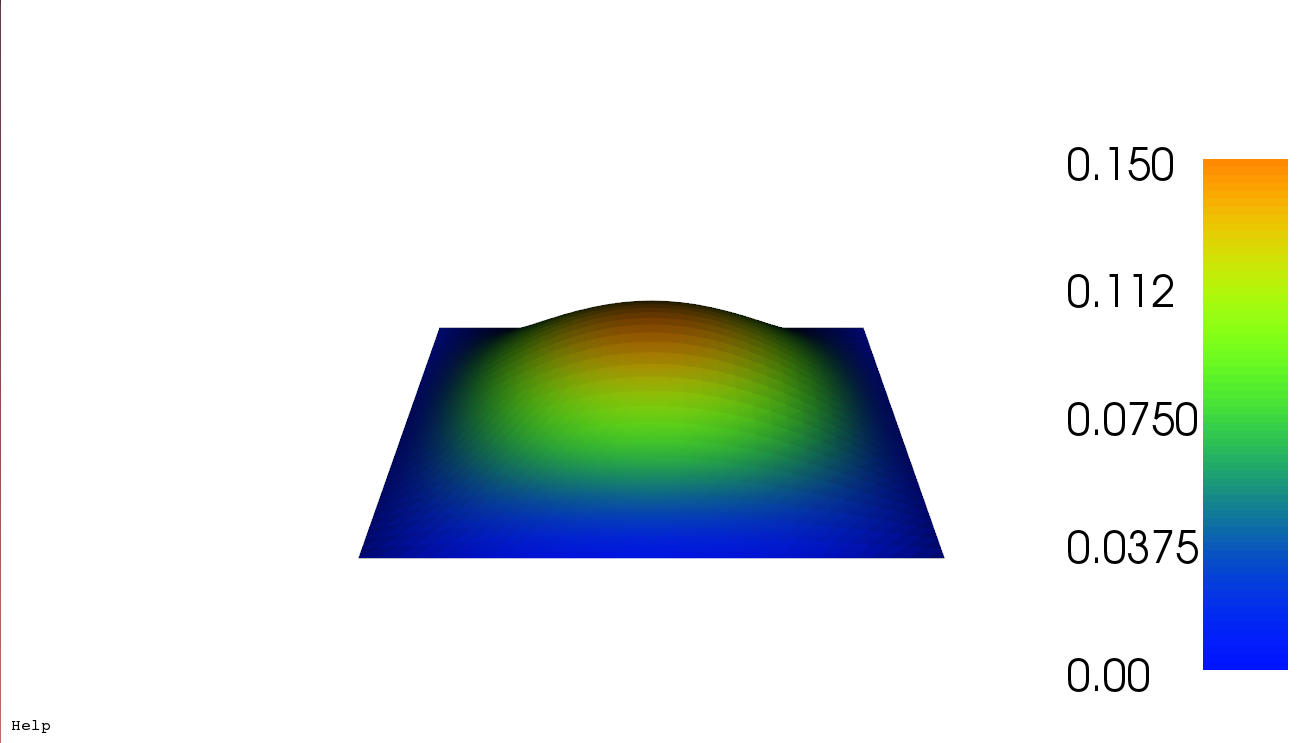
\includegraphics[scale = 0.25]{images/1024.png}
	\caption{$32 * 32$ elements}
\end{figure}

\end{document}
